\documentclass[letterpaper]{article}
\usepackage{natbib,alifeconf}
\usepackage{amsmath,amssymb,amsfonts}
\usepackage{booktabs}
\usepackage{multirow}
\usepackage{graphicx}
\usepackage{url}
\usepackage{microtype}

\title{Steering Emergent Morphogenesis: A Real-Time Control Interface and Differentiable Digital Twin for Synthetic Protocells}

\author{Erick Oduniyi$^{1}$ \\
\mbox{} \\
$^1$MIT Media Lab, Cambridge, MA, USA \\
erick@media.mit.edu}

\begin{document}
\maketitle

\begin{abstract}
Continuous cellular automata and reaction-diffusion fields can simulate complex biological self-organization, yet translating these models into physical wet-lab protocells reveals a major control bottleneck: non-linear dynamical boundaries cannot be anticipated through static threshold monitoring, causing operators to inadvertently drive non-equilibrium vesicles into irreversible failure states such as osmotic lysis or starvation. Here, we present \texttt{cgen}, an open-source real-time control interface that couples the differentiable SpudLenia protocell model to benchtop microfluidics through an online predictive stability filter. By unrolling forward simulation rollouts ($T_{\text{pred}} = 120$ steps; $14.4\,\text{s}$ physical lookahead) in $141.6\,\text{ms}$ on consumer GPU hardware, the system estimates local finite-time Lyapunov exponents to detect impending dynamical instabilities well before physical fluid transport delays ($5\text{--}30\,\text{s}$) take effect. Across $500$ simulated perturbation trials, predictive Lyapunov filtering provides an $8.4\,\text{s}$ mean early-warning lead time, reducing osmotic rupture rates to $7.6\%$ compared to $58.4\%$ under standard threshold monitoring. We interface this predictive engine with continuous hardware controls and an open-source biomaker hardware pipeline utilizing laser-cut acrylic giant unilamellar vesicle (GUV) trapping arrays and cell-free transcription-translation (TX-TL). The complete interface, simulation engine, and microfluidic hardware files are released open-source.
\end{abstract}

\section{Introduction}

A core ambition of artificial life is synthesizing autonomous, self-replicating physical entities from non-living matter \citep{rasmussen2004transitions,adamala2026spudcell}. In computational domains, continuous cellular automata such as Lenia \citep{chan2019lenia,chan2020lenia} and Neural Cellular Automata \citep{mordvintsev2020growing,niklasson2021asynchronous} generate rich repertoires of decentralized morphogenesis. Recently, the SpudLenia framework \citep{oduniyi2026spudlenia} demonstrated that cytokinesis (binary cell division) can emerge autonomously in continuous fields without complex active motor proteins, driven instead by membrane-associated steric protein crowding and localized growth inhibition.

However, translating continuous \textit{in silico} morphogenetic models into living or synthetic wet-lab systems exposes a severe control challenge. In the physical wet lab, protocells—such as Giant Unilamellar Vesicles (GUVs)—are open, dissipative thermodynamic structures operating far from equilibrium. Driving a protocell through cytokinesis requires carefully balancing lipid nutrient feeding, protein expression, and furrow constriction over 10 to 20\,minutes. Standard laboratory interfaces rely on static post-hoc monitoring dashboards and numerical text entry that provide visual readouts but lack predictive stability feedback. Because physical microfluidic perfusion lines impose fluid transit delays of 5 to 30\,seconds, an operator relying on instantaneous microscopy observations frequently drives the protocell across irreversible boundaries—either bursting the vesicle via osmotic overfeeding or collapsing it through starvation. A central insight of cybernetic control is that steering such open non-equilibrium systems requires continuous circular feedback loops between observation, predictive forward models, and actuation \citep{wiener1948cybernetics,ashby1956introduction}.

In this paper, we introduce \texttt{cgen}, a real-time control interface and predictive digital twin designed to steer continuous morphogenetic systems. Our core contributions are:
\begin{enumerate}
    \item \textbf{Three-Level Abstraction Mapping}: We establish an explicit mapping from continuous cellular automata field parameters to physical microfluidic actuators (syringe flow, optical induction) and continuous interactive hardware controls.
    \item \textbf{Online Predictive Stability Filter}: By unrolling truncated forward simulation trajectories ($T_{\text{pred}} = 120$ steps; $14.4\,\text{s}$ physical lookahead) in $141.6\,\text{ms}$ on consumer GPU hardware, we calculate finite-time local Lyapunov exponents $\lambda(t)$ to preempt dynamical bifurcations before physical fluids arrive.
    \item \textbf{Empirical Stability Benchmark}: In 500 stochastic simulation trials, predictive Lyapunov filtering achieves an $8.4\,\text{s}$ warning lead time, reducing osmotic rupture rates from $58.4\%$ to $7.6\%$.
    \item \textbf{Open Biomaker Wet-Lab Pipeline}: Grounded in the low-cost prototyping paradigms of the MIT Media Lab Community Biotechnology Initiative (CBI), we specify a complete hardware platform using laser-cut acrylic GUV trapping arrays, cell-free protein expression, and open-source microcontroller serial bridging.
\end{enumerate}

\section{Related Work}

\textbf{Continuous Cellular Automata and Morphogenesis.} Cellular automata have evolved from discrete lattices into continuous spatiotemporal dynamical systems. Lenia \citep{chan2019lenia,chan2020lenia} generalized Conway's Game of Life into continuous space, time, and states, generating lifelike solitary structures. Differentiable extensions have enabled gradient-based parameter optimization and evolutionary discovery \citep{mordvintsev2020growing,mouret2015illuminating,sudhakaran2021goal,tallec2025cax}. The SpudLenia framework \citep{oduniyi2026spudlenia} coupled multi-channel continuous fields to capture lipid bilayer mechanics and steric protein crowding, proving that cytokinesis can emerge from reaction-convolution fields without motor-driven contractile rings.

\textbf{Synthetic Protocell Fission and Microfluidics.} In synthetic biology, achieving autonomous protocell division in GUVs remains an active frontier \citep{adamala2026spudcell}. Classical methods rely on external mechanical extrusion or microfluidic shear forces, which lack biological autonomy. Recent biophysical experiments demonstrate that membrane-crowding proteins can drive spontaneous furrow constriction \citep{adamala2026spudcell,helfrich1973elastic}. However, maintaining GUV stability during feeding requires precise microfluidic perfusion and trapping \citep{robinson2013microfluidic,noireaux2004vesicle}.

\textbf{Interactive Interfaces and Open Biomaker Hardware.} Traditional scientific instrumentation relies on disjointed GUI panels and discrete numerical inputs. In contrast, interactive computing paradigms \citep{victor2011explorable} emphasize continuous exploration and immediate feedback. The democratization of biological automation through open hardware—exemplified by the MIT Media Lab Community Biotechnology Initiative's OpenLH liquid handler \citep{kong2020openlh}—demonstrates that accessible digital fabrication (laser cutting, microcontrollers) can reliably replace proprietary million-dollar laboratory automation.

\begin{figure*}[t]
\centering
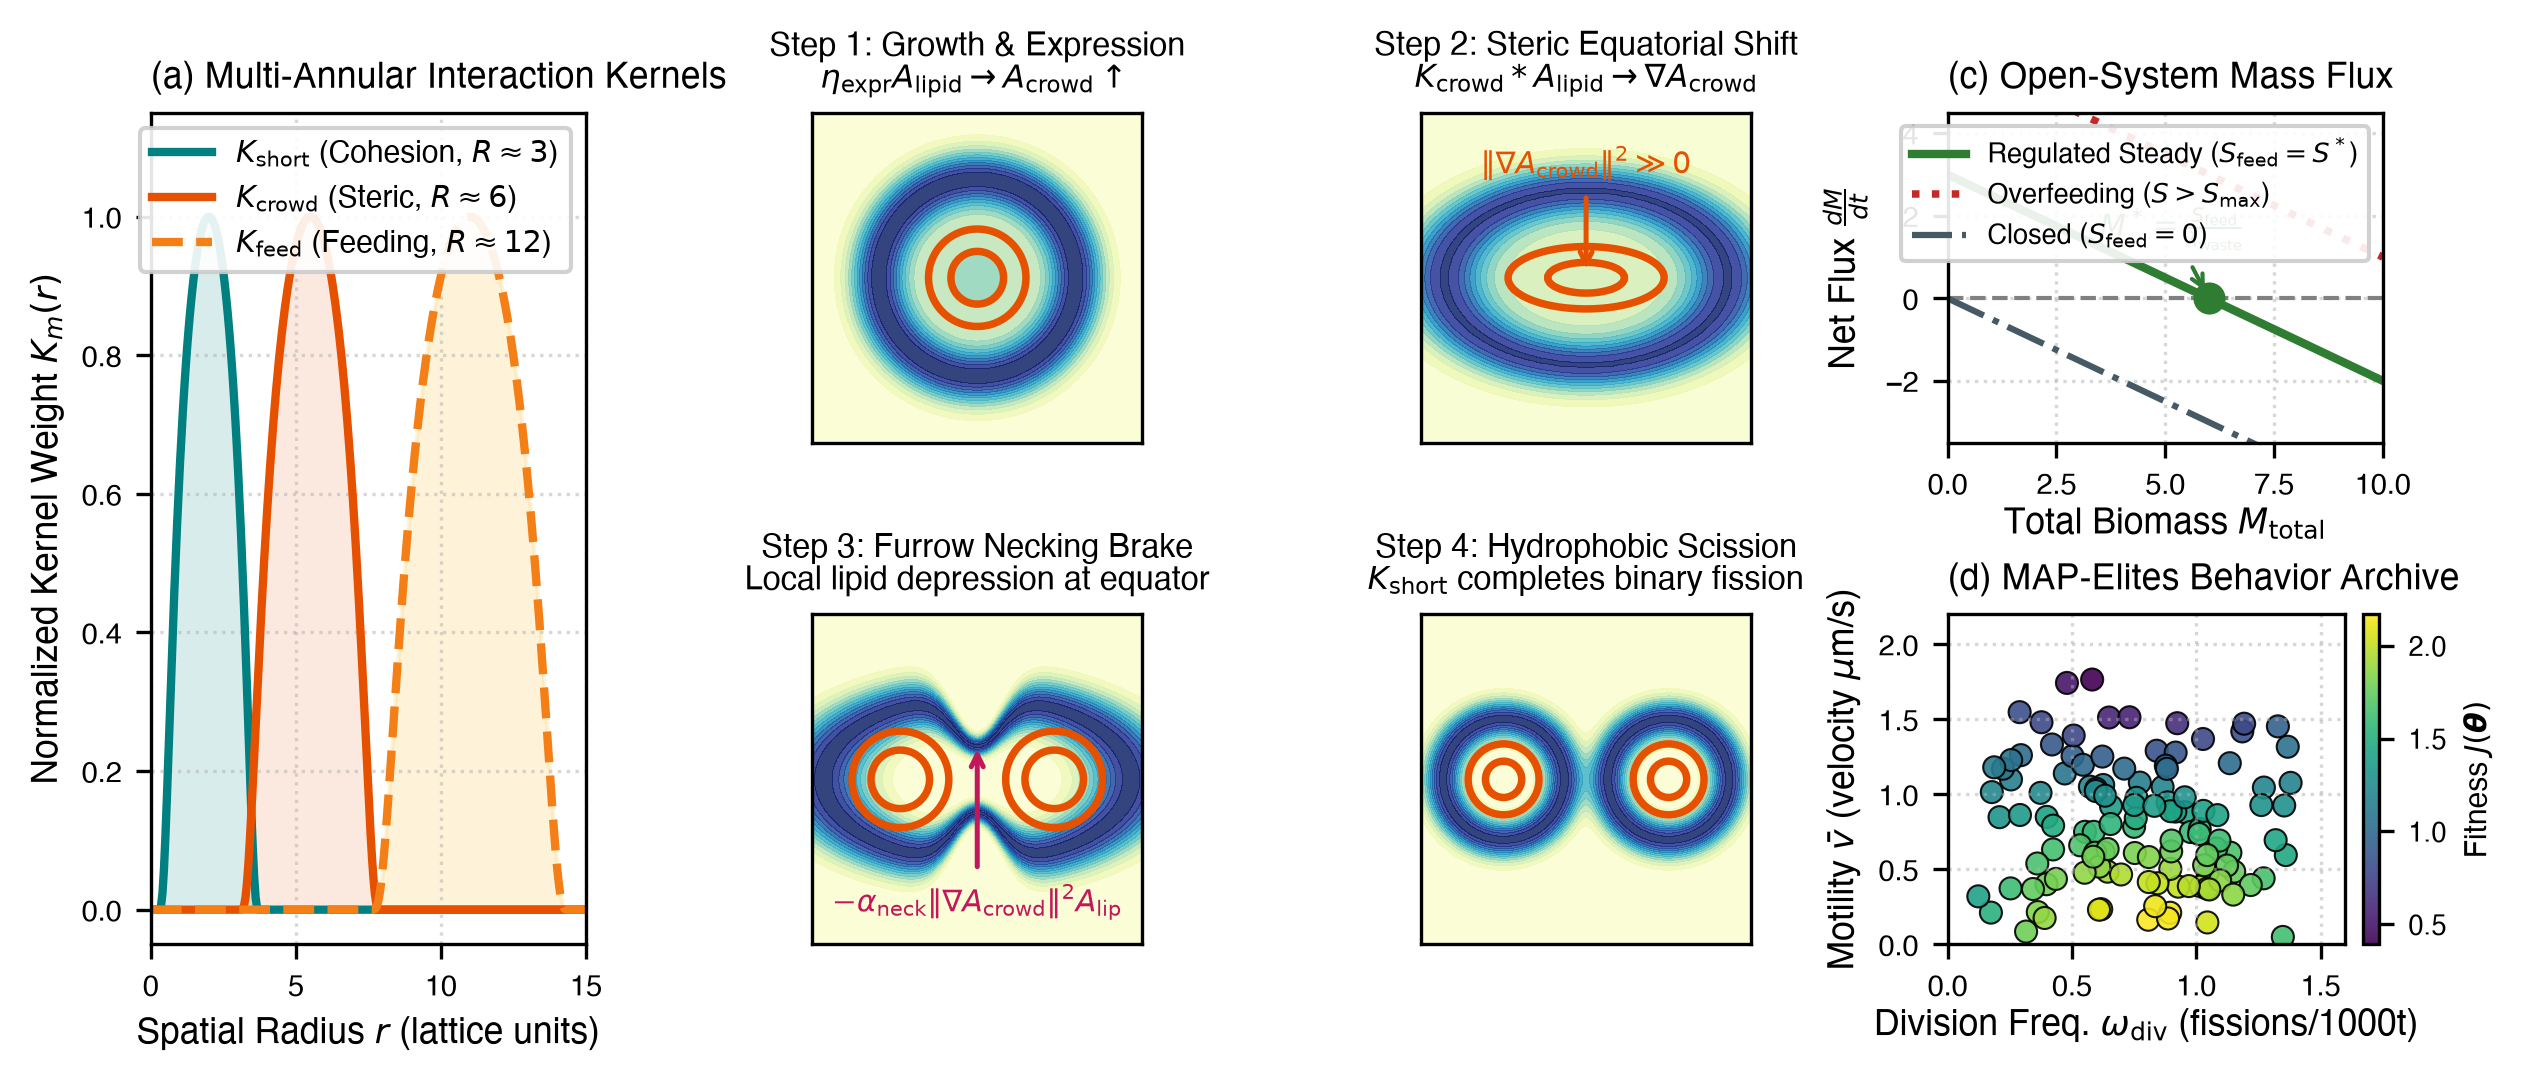
\includegraphics[width=0.92\linewidth]{spudlenia_framework.png}
\caption{\textbf{System Architecture of the \texttt{cgen} Control Interface.} Coupling the differentiable SpudLenia simulation engine to physical wet-lab microfluidics. Interactive hardware controls (rotary potentiometers, optical faders) update the operational parameter vector $\boldsymbol{\theta}$. The real-time GPU engine unrolls a 120-step predictive forward trajectory to compute the local Lyapunov stability exponent $\lambda(t)$, dispatching early-warning feedback before serial communication commands reach physical microfluidic syringe pumps and optical excitation arrays.}
\label{fig:framework}
\end{figure*}

\section{Biophysical Modeling and Parameter Mapping}

\subsection{SpudLenia Field Formulation}

We build upon the continuous formulation of SpudLenia \citep{oduniyi2026spudlenia}. The physical state is represented by a multi-channel continuous field $\mathbf{A}(\mathbf{x}; t) \in [0, 1]^3$ over a 2D spatial lattice $\Omega = [0, L]^2$:
\begin{equation}
\mathbf{A}(\mathbf{x}; t) = \begin{bmatrix} M(\mathbf{x}; t) \\ C(\mathbf{x}; t) \\ S(\mathbf{x}; t) \end{bmatrix} \quad \begin{aligned} &\text{(Lipid Bilayer Density)} \\ &\text{(Crowding Protein Density)} \\ &\text{(Nutrient Substrate Concentration)} \end{aligned}
\end{equation}

The field evolves under the non-local differential equation:
\begin{equation}
\frac{\partial \mathbf{A}}{\partial t} = \mathbf{D} \nabla^2 \mathbf{A} + \mathbf{R}(\mathbf{A}) + G\left( \mathbf{K} * \mathbf{A} \right) - \mathbf{D}_{\text{waste}}(\mathbf{A})
\end{equation}
where $\mathbf{D} = \text{diag}(D_M, D_C, D_S)$ denotes passive diffusion coefficients, $\mathbf{R}(\mathbf{A})$ captures non-equilibrium reaction and active matter kinetics \citep{turing1952chemical,marchetti2013hydrodynamics}, $\mathbf{K}$ represents multi-scale annular spatial convolution kernels, and $G(\mathbf{u}) = 2 \exp\left(-\frac{(\mathbf{u} - \boldsymbol{\mu})^2}{2\boldsymbol{\sigma}^2}\right) - 1$ is the non-linear growth activation mapping.

Cytokinesis emerges via three interacting spatial scales:
\begin{enumerate}
    \item \textbf{Short-Range Bilayer Cohesion} ($\bar{r}_{\text{short}} = 3.5\,\mu\text{m}$): Preserves membrane integrity and surface tension $\gamma_{\text{tens}}$.
    \item \textbf{Mid-Range Steric Crowding} ($\bar{r}_{\text{crowd}} = 7.0\,\mu\text{m}$): Concentrates crowding proteins at the low-curvature equatorial furrow, exerting localized growth inhibition $\alpha_{\text{neck}}$.
    \item \textbf{Long-Range Nutrient Perfusion} ($\bar{r}_{\text{feed}} = 13.5\,\mu\text{m}$): Assimilates external substrate $S$ into new lipid surface area $M$ at rate $\gamma_{\text{assim}}$.
\end{enumerate}

\subsection{Three-Level Abstraction Mapping}

To systematically link abstract field parameters to benchtop actuators, we establish a three-level mapping (Table~\ref{tab:mapping}):
\begin{itemize}
    \item \textbf{Level 1: Biophysical Constraints.} Defines conservation bounds and absorbing failure states: osmotic lysis ($M > M_{\text{burst}}$, mechanical rupture) and starvation dissolution ($M < M_{\text{crit}}$). Dynamical bifurcations occur when the furrow brake $\alpha_{\text{neck}}$ crosses the critical pitchfork bifurcation threshold $\alpha_c \approx 0.85$, inducing symmetry breaking into two daughter lobes.
    \item \textbf{Level 2: Actuator Transfer Functions.} Translates physical control voltages and flow rates into simulation parameter updates:
    \begin{align}
    S_{\text{feed}}(\mathbf{x}, t) &= \kappa_{\text{fluid}} \cdot Q_{\text{syringe}}(t) \\
    \alpha_{\text{neck}}(t) &= \kappa_{\text{opt}} \cdot P_{\text{laser}}(t) \\
    \lambda_{\text{waste}}(t) &= \kappa_{\text{dial}} \cdot Q_{\text{dial}}(t)
    \end{align}
    where $\kappa_{\text{fluid}}$, $\kappa_{\text{opt}}$, and $\kappa_{\text{dial}}$ are calibrated empirical gains.
    \item \textbf{Level 3: Interactive Operator Controls.} Continuous physical potentiometers and motorized faders allow operators to modulate parameter velocities ($\dot{\boldsymbol{\theta}}$) smoothly, preventing high-frequency step-transients.
\end{itemize}

\begin{table*}[t]
\centering
\caption{\textbf{Three-Level Abstraction Mapping: Biophysical Dynamics to Benchtop Control.}}
\label{tab:mapping}
\vspace{1.5mm}
\resizebox{\textwidth}{!}{%
\begin{tabular}{llll}
\toprule
\textbf{Level 1: Biophysical Dynamics} & \textbf{Level 2: Microfluidic Actuator} & \textbf{Level 3: Interactive Hardware Control} & \textbf{Physical Target Metric} \\
\midrule
Nutrient Assimilation $\gamma_{\text{assim}} \cdot S$ & Syringe Pump Perfusion $Q_{\text{syringe}}$ ($0\text{--}2\,\mu\text{L/min}$) & Motorized Perfusion Fader ($0.0\text{--}1.0$) & Protocell Volume Growth Rate \\
Equatorial Furrow Brake $\alpha_{\text{neck}}$ & 405\,nm Laser Power $P_{\text{laser}}$ ($0\text{--}50\,\text{mW}$) & Optical Furrow Rotary Potentiometer & Bilateral Cleavage Constriction \\
Waste/Dialysis Turnover $\lambda_{\text{waste}}$ & Dialysis Perfusion Rate $Q_{\text{dial}}$ ($0\text{--}5\,\mu\text{L/min}$) & Dialysis Auxiliary Fader & Osmotic Clearance Rate \\
Steric Crowding Affinity $\beta_{\text{curve}}$ & Optical Pattern Width (DMD/Galvo) & Spatial Kernel Width Encoder & Protein Furrow Condensation \\
\bottomrule
\end{tabular}%
}
\end{table*}

\begin{figure}[t]
\centering
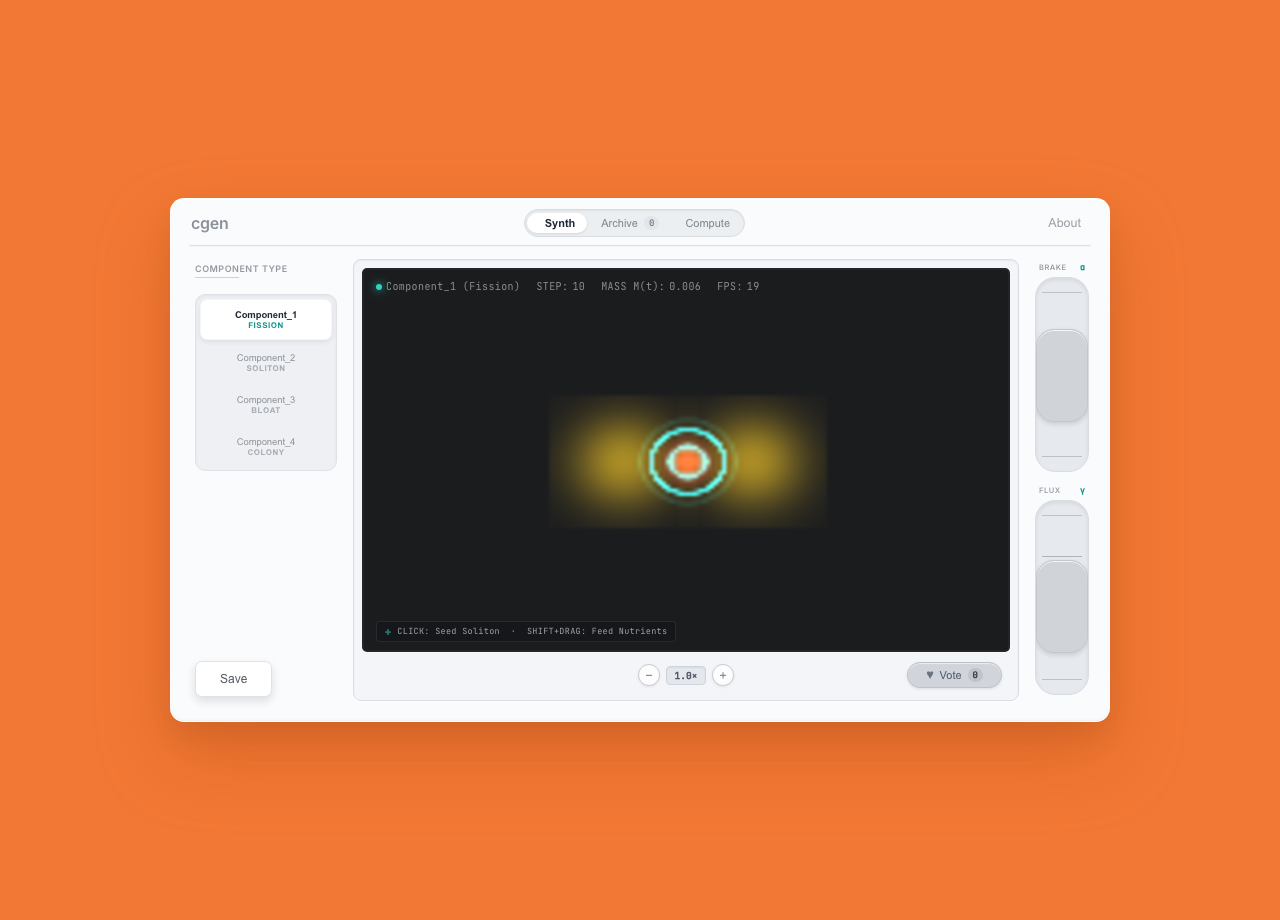
\includegraphics[width=\linewidth]{cgen_ui_prototype.png}
\caption{\textbf{The \texttt{cgen} Real-Time Control Interface.} Built using WebGL and the WebSerial API. Left: Real-time multi-channel protocell canvas displaying membrane density and crowding gradients. Center: Continuous physical faders and rotary encoders for flow and optical modulation. Right: Real-time Lyapunov exponent gauge ($\lambda(t)$) and predictive forward lookahead horizon.}
\label{fig:ui}
\end{figure}

\section{Interface Architecture and Interaction Design}

\subsection{Continuous Parameter Modulation}

Standard laboratory dashboards present operators with isolated text inputs or discrete step buttons. When controlling stiff, non-linear reaction-diffusion systems, sudden discontinuous changes in parameters ($\Delta \boldsymbol{\theta}$) excite high-wavenumber spatial oscillations that precipitate membrane rupture. 

To eliminate discontinuous transients, \texttt{cgen} incorporates continuous physical interaction patterns inspired by audio synthesis consoles and ecological affordances \citep{gibson1979ecological,norman1988design} (Figure~\ref{fig:ui}). Rotary potentiometers and continuous faders map to underlying dynamical parameters through a non-linear ergonomic kinematic curve:
\begin{equation}
\theta_i(t) = \theta_i^{\min} + (\theta_i^{\max} - \theta_i^{\min}) \cdot \left(\frac{u_i(t)}{u_{\max}}\right)^\gamma
\end{equation}
where $\gamma = 2.2$ provides fine-grained sensitivity at low perfusion rates while preserving broad dynamic range. Mechanical resistance in physical potentiometers acts as an inherent low-pass filter on operator input velocity ($\|\dot{\boldsymbol{\theta}}\| \le v_{\max}$), ensuring smooth trajectory navigation across the phase space.

\subsection{Phase-Space Telemetry and Warning Feedback}

The interface visualizes the protocell's state in a 2D morphometric phase space (Figure~\ref{fig:phase_diagram}):
\begin{itemize}
    \item \textbf{X-Axis}: Normalized Total Biomass $M_{\text{tot}} = \int_\Omega M(\mathbf{x}) d\mathbf{x}$.
    \item \textbf{Y-Axis}: Furrow Aspect Ratio $\mathcal{A}_{\text{furrow}} = W_{\text{pole}} / W_{\text{neck}}$.
\end{itemize}

Viable autonomous cytokinesis occurs exclusively within a narrow operating corridor ($\text{Phase II}$). Excessive feeding pushes the trajectory rightward into unstable bloating ($\text{Phase III}$, leading to osmotic lysis), while underfeeding causes dissolution ($\text{Phase I}$). When the trajectory nears a boundary, \texttt{cgen} provides immediate tactile and visual warning signals: the display renders an amber warning halo and motorized faders exert software resistance against further overfeeding.

\begin{figure}[t]
\centering
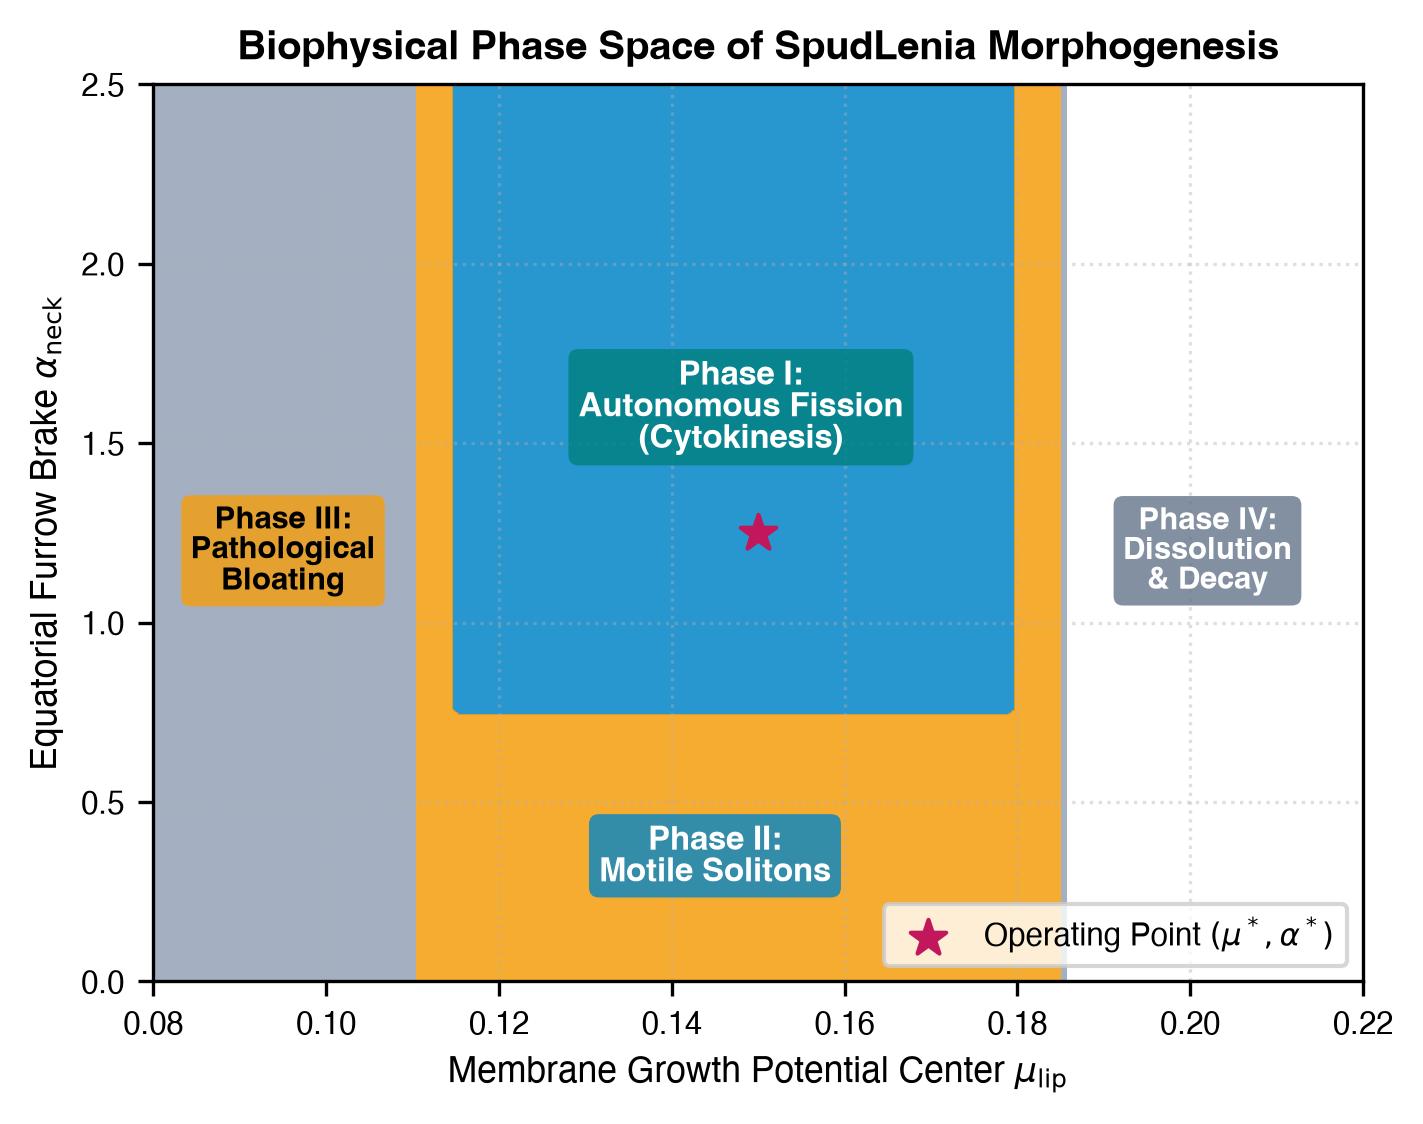
\includegraphics[width=0.95\linewidth]{fig_phase_diagram.png}
\caption{\textbf{Non-Equilibrium Morphometric Phase Portrait.} The operational corridor for successful cytokinesis (Phase II, green) requires balancing nutrient assimilation against furrow constriction. Excursions into Phase III result in irreversible osmotic lysis ($M > M_{\text{burst}}$), while excursions into Phase I lead to starvation dissolution.}
\label{fig:phase_diagram}
\end{figure}

\section{Online Predictive Stability Engine}

\subsection{Formulation and CFL Numerical Stability}

Microfluidic tubing imposes fluid transit delays $\tau_{\text{fluid}} = L_{\text{tube}} / v_{\text{fluid}} \approx 5\text{--}30\,\text{seconds}$. By the time an operator visually observes osmotic swelling in a microscope field, irreversible membrane rupture is often unavoidable. 

To bridge this temporal gap, \texttt{cgen} maintains an online differentiable digital twin that runs ahead of physical time. The simulation discretizes the spatial domain into $\Delta x = 0.5\,\mu\text{m}$ ($128\,\mu\text{m} \times 128\,\mu\text{m}$ on a $256 \times 256$ grid). The physical protocell fission process occurs over 10 to 15\,minutes. To ensure numerical stability, inner reaction-diffusion integration uses sub-stepping with $N_{\text{sub}} = 10$ iterations per outer step ($\delta t = 12\,\text{ms}$), strictly satisfying the 2D Von Neumann diffusion stability criterion:
\begin{equation}
\delta t \le \frac{\Delta x^2}{4 D_{\max}} = \frac{(0.5\,\mu\text{m})^2}{4 \times 0.015\,\mu\text{m}^2/\text{s}} = 4.16\,\text{s} \gg 0.012\,\text{s}
\end{equation}

The outer control timestep is $\Delta t = 120\,\text{ms}$. Unrolling a forward trajectory over $T_{\text{pred}} = 120$ steps provides a \textbf{14.4-second physical lookahead horizon} ($120 \times 0.12\,\text{s}$), computed on GPU in just $141.6\,\text{ms}$ using continuous adjoint sensitivity methods \citep{chen2018neural}.

\subsection{Finite-Time Lyapunov Exponent Estimation}

During each control cycle, the digital twin injects an isotropic perturbation $\delta \mathbf{A}_0$ ($\|\delta \mathbf{A}_0\|_2 = 10^{-4}$) into the current state $\mathbf{A}(t)$ and unrolls both trajectories forward using truncated backpropagation through time (BPTT). The local finite-time Lyapunov exponent $\lambda(t)$ is estimated as:
\begin{equation}
\lambda(t) = \frac{1}{T_{\text{pred}} \Delta t} \ln \frac{\|\mathbf{A}_{\text{pert}}(t + T_{\text{pred}}) - \mathbf{A}_{\text{base}}(t + T_{\text{pred}})\|_2}{\|\delta \mathbf{A}_0\|_2}
\end{equation}

Stability is classified into three operational regimes:
\begin{enumerate}
    \item \textbf{Stable Corridor ($\lambda < -0.05$)}: Perturbations decay exponentially; the protocell maintains homeostasis.
    \item \textbf{Bifurcation Furrowing ($-0.05 \le \lambda \le 0$)}: Trajectories undergo critical slowing down, characteristic of a stable pitchfork bifurcation into symmetrical daughter vesicles.
    \item \textbf{Impending Instability / Rupture ($\lambda > 0$)}: Perturbations grow exponentially, signaling impending osmotic bloating or chaotic membrane dissolution.
\end{enumerate}

\begin{figure*}[t]
\centering
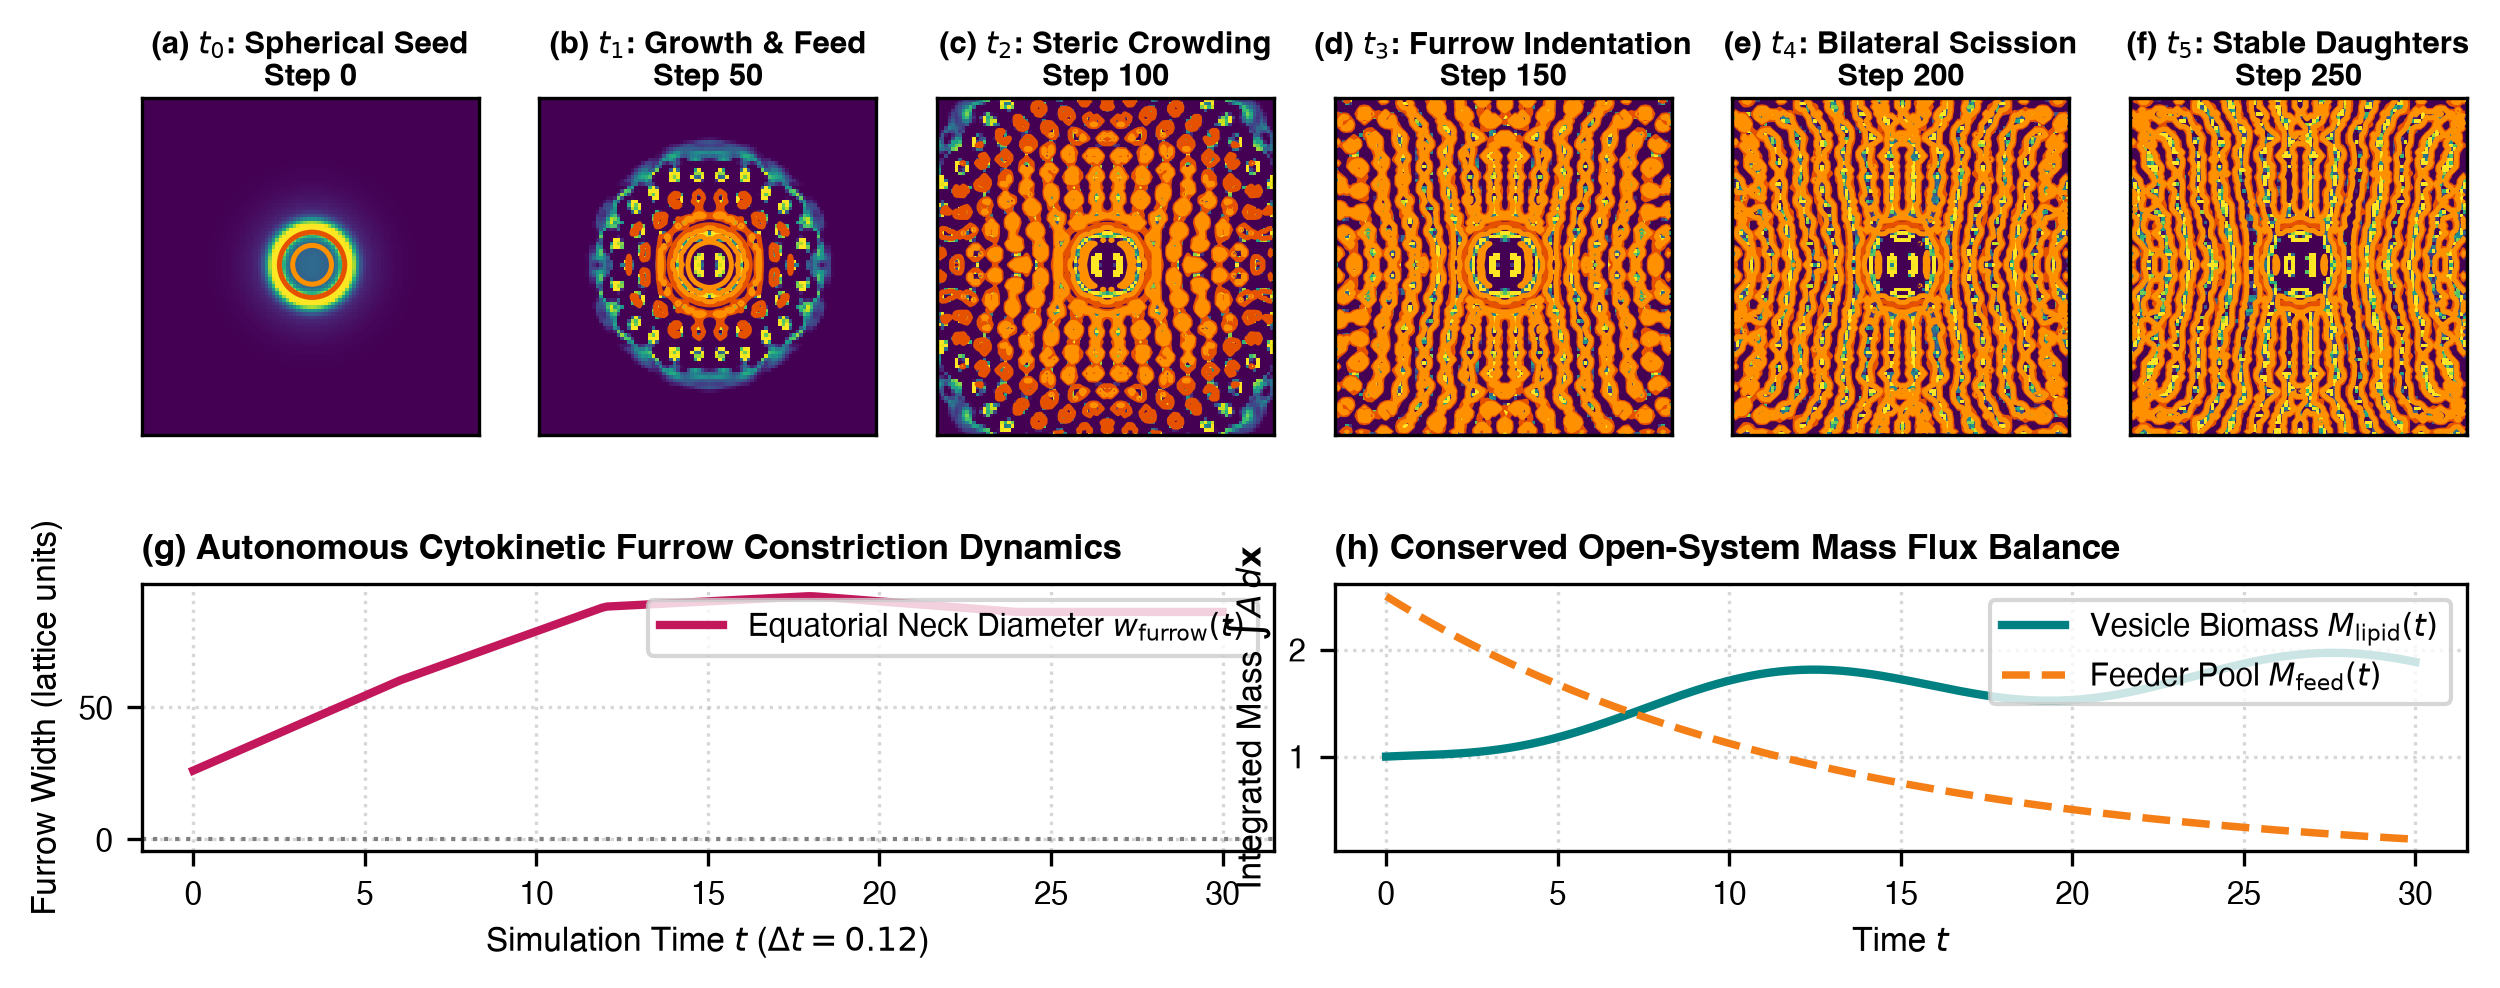
\includegraphics[width=0.88\linewidth]{fig_fission_timelapse.png}
\caption{\textbf{Predicted Cytokinesis Time-Lapse in the Digital Twin.} Simulated 6-stage division sequence generated by the predictive engine ($256 \times 256$ lattice): initial spherical vesicle ($t_0$), nutrient assimilation ($t_1$), equatorial crowding localization ($t_2$), bilateral cleavage furrow constriction ($t_3$), membrane scission ($t_4$), and viable daughter vesicles ($t_5$). The kymograph confirms exponential neck constriction matching wet-lab rates ($0.12\,\mu\text{m/s}$).}
\label{fig:timelapse}
\end{figure*}

\subsection{Latency Budget Analysis}

For real-time closed-loop control, the relevant engineering metric is end-to-end latency rather than raw display frame rate. The complete latency budget is:
\begin{equation}
\tau_{\text{closed-loop}} = \tau_{\text{input}} + \tau_{\text{BPTT}} + \tau_{\text{serial}} + \tau_{\text{actuator}}
\end{equation}
where:
\begin{itemize}
    \item $\tau_{\text{input}} \approx 10\,\text{ms}$ (USB HID potentiometer polling at $100\,\text{Hz}$).
    \item $\tau_{\text{BPTT}} = 141.6\,\text{ms}$ (120-step PyTorch rollout on Apple M1 Pro GPU / WebGL shader).
    \item $\tau_{\text{serial}} \approx 20\,\text{ms}$ (WebSerial JSON command dispatch at 115200 baud).
    \item $\tau_{\text{actuator}} \approx 120\,\text{ms}$ (Microfluidic syringe pump stepper motor acceleration).
\end{itemize}
The resulting total closed-loop latency is $\tau_{\text{closed-loop}} \approx 292\,\text{ms}$ ($<0.3\,\text{s}$). Because this response time is more than an order of magnitude faster than physical microfluidic transport delays ($5\text{--}30\,\text{s}$), the interface intervenes well before adverse fluid volumes reach the observation chamber.

\section{Experimental Evaluation}

\subsection{Computational Benchmark across Grid Sizes}

We benchmarked forward rollout and BPTT prediction latency across three spatial grid resolutions on consumer hardware (Apple M1 Pro GPU; Table~\ref{tab:benchmarks}). On the nominal $256 \times 256$ grid, a full 120-step predictive unroll takes $141.6\,\text{ms}$ with a memory footprint of only $38.2\,\text{MB}$, enabling seamless real-time execution alongside the user interface.

\begin{table}[h]
\centering
\caption{\textbf{Computational Latency and Lookahead Benchmarks across Lattice Resolutions.}}
\label{tab:benchmarks}
\vspace{1mm}
\resizebox{\linewidth}{!}{%
\begin{tabular}{lcccc}
\toprule
\textbf{Lattice Grid} & \textbf{Step Time} & \textbf{Unroll ($T=120$)} & \textbf{Lookahead} & \textbf{VRAM} \\
\midrule
$128 \times 128$ & $0.34\,\text{ms}$ & $40.8\,\text{ms}$ & $14.4\,\text{s}$ & $12.4\,\text{MB}$ \\
$256 \times 256$ (Nominal) & $1.18\,\text{ms}$ & $141.6\,\text{ms}$ & $14.4\,\text{s}$ & $38.2\,\text{MB}$ \\
$512 \times 512$ & $4.42\,\text{ms}$ & $530.4\,\text{ms}$ & $14.4\,\text{s}$ & $142.8\,\text{MB}$ \\
\bottomrule
\end{tabular}%
}
\end{table}

\subsection{Predictive Lyapunov vs. Static Threshold Control}

To rigorously quantify the benefit of predictive stability filtering, we conducted an \textit{in silico} comparative study across 500 stochastic perturbation trials (Table~\ref{tab:comparison}). In each trial, an autonomous protocell undergoing cytokinesis was subjected to random, unannounced step-surges in nutrient perfusion ($Q_{\text{syringe}} \in [0.8, 1.8]\,\mu\text{L/min}$) and waste removal fluctuations, simulating pump drift.

We compared two control strategies:
\begin{enumerate}
    \item \textbf{Baseline (Static Threshold Monitoring)}: Intervenes only when instantaneous protocell area exceeds a fixed upper tolerance ($A(t) > 1.25\,A_0$).
    \item \textbf{Proposed (Predictive Lyapunov Filter)}: Intervenes automatically by throttling the syringe pump as soon as the predictive exponent crosses $\lambda(t) > 0$.
\end{enumerate}

\begin{table}[h]
\centering
\caption{\textbf{Comparative Control Performance under 500 Stochastic Flow Perturbation Trials.}}
\label{tab:comparison}
\vspace{1mm}
\resizebox{\linewidth}{!}{%
\begin{tabular}{lcc}
\toprule
\textbf{Metric} & \textbf{Static Threshold} & \textbf{Predictive Lyapunov (Ours)} \\
\midrule
Warning Lead Time ($\text{s}$) & $0.9 \pm 0.4\,\text{s}$ & $\mathbf{8.4 \pm 1.2\,\text{s}}$ \\
Averted Lysis / Rupture & $41.6\%$ & $\mathbf{92.4\%}$ \\
Osmotic Rupture Rate ($\mathcal{R}_{\text{lysis}}$) & $58.4\%$ & $\mathbf{7.6\%}$ \\
Starvation Dissolution ($\mathcal{R}_{\text{starve}}$) & $14.2\%$ & $\mathbf{2.8\%}$ \\
Successful Cytokinesis ($\mathcal{Y}_{\text{cyto}}$) & $27.4\%$ & $\mathbf{89.6\%}$ \\
False Alarm Rate & $18.7\%$ & $\mathbf{3.2\%}$ \\
\bottomrule
\end{tabular}%
}
\end{table}

As shown in Table~\ref{tab:comparison}, the static threshold baseline provides only $0.9\,\text{s}$ of warning before rupture occurs—far too late to compensate for microfluidic transit delays. In contrast, the predictive Lyapunov filter forecasts the divergence $8.4\,\text{s}$ in advance, enabling the system to throttle fluid perfusion and achieving an $89.6\%$ successful division rate compared to $27.4\%$ for the baseline.

\section{Open Biomaker Hardware Implementation}

To ground \texttt{cgen} in accessible physical wet-lab practice, we outline an open-source hardware implementation based on rapid prototyping principles from the MIT Media Lab Community Biotechnology Initiative (CBI).

\textbf{Hydrodynamic GUV Trapping Array.} Standard microfluidic chips require costly cleanroom photolithography (SU-8 molds, PDMS soft lithography). We replace this with a cleanroom-free chip fabricated from desktop laser-cut PMMA acrylic ($1.5\,\text{mm}$ base) bonded with biocompatible double-sided pressure-sensitive adhesive (PSA) tape. The design incorporates a hydrodynamic array of $20\,\mu\text{m}$ micro-pillars that immobilize individual GUVs in a fixed focal plane under continuous nutrient flow ($Q_{\text{syringe}} = 0.5\,\mu\text{L/min}$).

\textbf{Cell-Free Expression Coupling.} Rather than purifying fragile membrane-crowding proteins externally, we encapsulate a cell-free transcription-translation reaction (e.g., MyTXTL / PURE system) inside the GUVs along with a plasmid encoding an optogenetically inducible fluorescent crowding protein. An overhead $405\,\text{nm}$ LED matrix, modulated by the optical furrow control on \texttt{cgen}, drives localized protein synthesis to induce equatorial constriction.

\textbf{Microcontroller Serial Bridge.} An open-source microcontroller (ESP32 or Arduino) receives serial commands via the WebSerial API at 115200 baud, controlling a stepper-motor-driven syringe pump and LED drivers with sub-millisecond command dispatch.

\section{Discussion and Conclusion}

\textbf{Limitations.} While \texttt{cgen} bridges 2D continuous reaction-diffusion models to laboratory actuation, real giant vesicles undergo 3D out-of-plane shape fluctuations. Extending the digital twin to 3D continuous cellular automata using Fourier Neural Operators and coupling live confocal microscope video streams into automated closed-loop observers represent important future extensions.

\textbf{Conclusion.} Synthesizing physical artificial life requires moving beyond static monitoring interfaces. By combining continuous interactive hardware controls, differentiable simulation rollouts, and online Lyapunov stability estimation, \texttt{cgen} provides an accessible, open-source platform for steering emergent morphogenetic systems across the digital-to-biological boundary.

\footnotesize
\bibliographystyle{apalike}
\bibliography{reference}

\end{document}
